\documentclass[10pt]{article}
\usepackage[utf8]{inputenc}
\usepackage[T1]{fontenc}
\usepackage{amsmath}
\usepackage{amsfonts}
\usepackage{amssymb}
\usepackage[version=4]{mhchem}
\usepackage{stmaryrd}
\usepackage{bbold}
\usepackage{graphicx}
\usepackage[export]{adjustbox}
\graphicspath{ {./images/} }

\title{Machine Learning Course - CS-433 
 K-Means Clustering }

\author{}
\date{}


\begin{document}
\maketitle
Nov 22, 2023

Martin Jaggi

Last updated on: November 20, 2023

credits to Mohammad Emtiyaz Khan \& Rüdiger Urbanke

EPFL

\section*{Clustering}
Clusters are groups of points whose inter-point distances are small compared to the distances outside the cluster.

The goal is to find "prototype" points $\boldsymbol{\mu}_{1}, \boldsymbol{\mu}_{2}, \ldots, \boldsymbol{\mu}_{K}$ and cluster assignments $z_{n} \in\{1,2, \ldots, K\}$ for all $n=1,2, \ldots, N$ data vectors $\mathbf{x}_{n} \in \mathbb{R}^{D}$.

\section*{$\mathrm{K}$-means clustering}
Assume $K$ is known.

$$
\min _{\mathbf{z}, \boldsymbol{\mu}} \mathcal{L}(\mathbf{z}, \boldsymbol{\mu})=\sum_{n=1}^{N} \sum_{k=1}^{K} z_{n k}\left\|\mathbf{x}_{n}-\boldsymbol{\mu}_{k}\right\|_{2}^{2}
$$

s.t. $\boldsymbol{\mu}_{k} \in \mathbb{R}^{D}, z_{n k} \in\{0,1\}, \sum_{k=1}^{K} z_{n k}=1$,

where $\mathbf{z}_{n}=\left[z_{n 1}, z_{n 2}, \ldots, z_{n K}\right]^{\top}$

$$
\begin{aligned}
\mathbf{z} & =\left[\mathbf{z}_{1}, \mathbf{z}_{2}, \ldots, \mathbf{z}_{N}\right]^{\top} \\
\boldsymbol{\mu} & =\left[\boldsymbol{\mu}_{1}, \boldsymbol{\mu}_{2}, \ldots, \boldsymbol{\mu}_{K}\right]^{\top}
\end{aligned}
$$

Is this optimization problem easy?

Algorithm: Initialize $\boldsymbol{\mu}_{k} \forall k$,

then iterate:

\begin{enumerate}
  \item For all $n$, compute $\mathbf{z}_{n}$ given $\boldsymbol{\mu}$.

  \item For all $k$, compute $\boldsymbol{\mu}_{k}$ given $\mathbf{z}$.

\end{enumerate}

Step 1: For all $n$, compute $\mathbf{z}_{n}$ given $\boldsymbol{\mu}$.
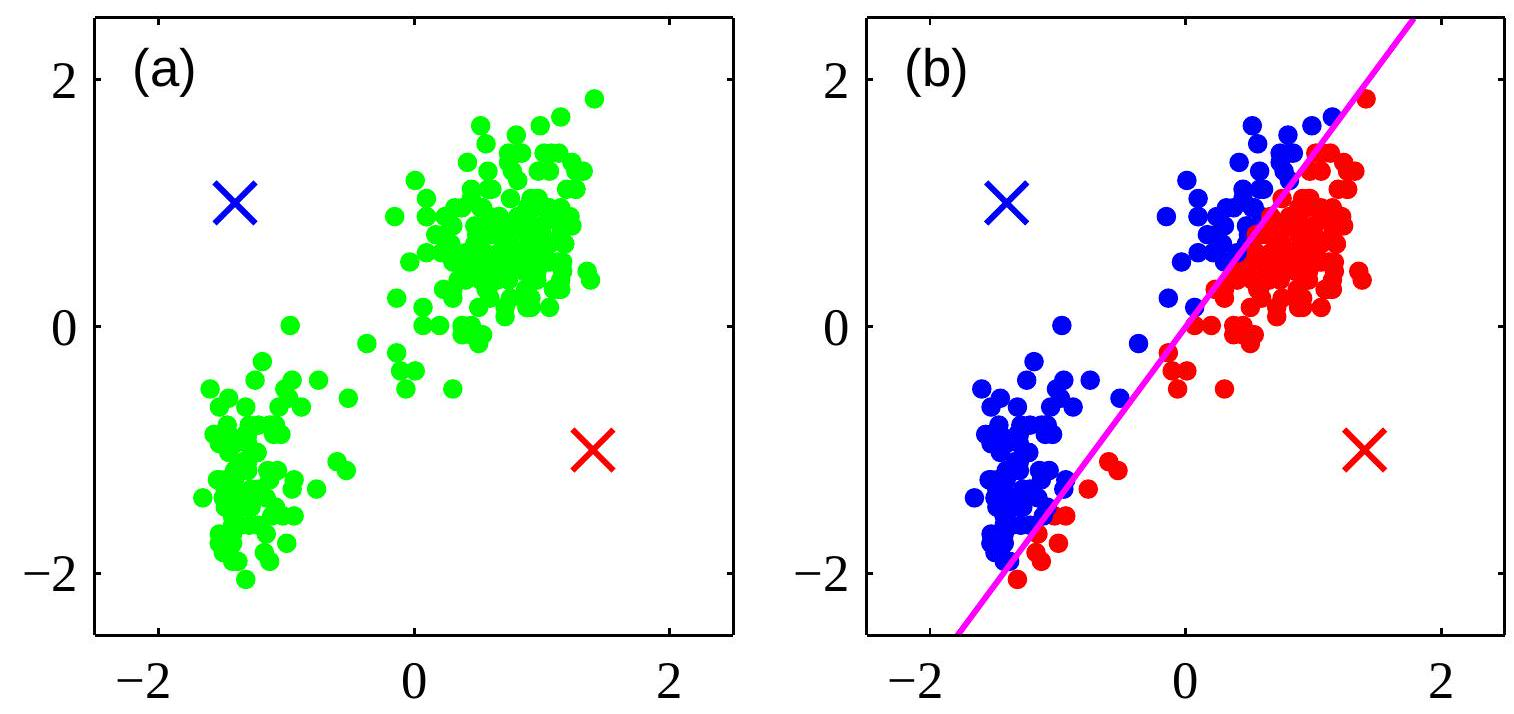
\includegraphics[max width=\textwidth, center]{2023_12_30_43b7e6c218cb987b5fcag-3}

$z_{n k}=\left\{\begin{array}{l}1 \text { if } k=\arg \min _{j=1,2, \ldots K}\left\|\mathbf{x}_{n}-\boldsymbol{\mu}_{j}\right\|_{2}^{2} \\ 0 \text { otherwise }\end{array}\right.$

Step 2: For all $k$, compute $\boldsymbol{\mu}_{k}$ given $\mathbf{z}$.

Take derivative w.r.t. $\boldsymbol{\mu}_{k}$ to get:

$$
\boldsymbol{\mu}_{k}=\frac{\sum_{n=1}^{N} z_{n k} \mathbf{x}_{n}}{\sum_{n=1}^{N} z_{n k}}
$$

Hence, the name 'K-means'.
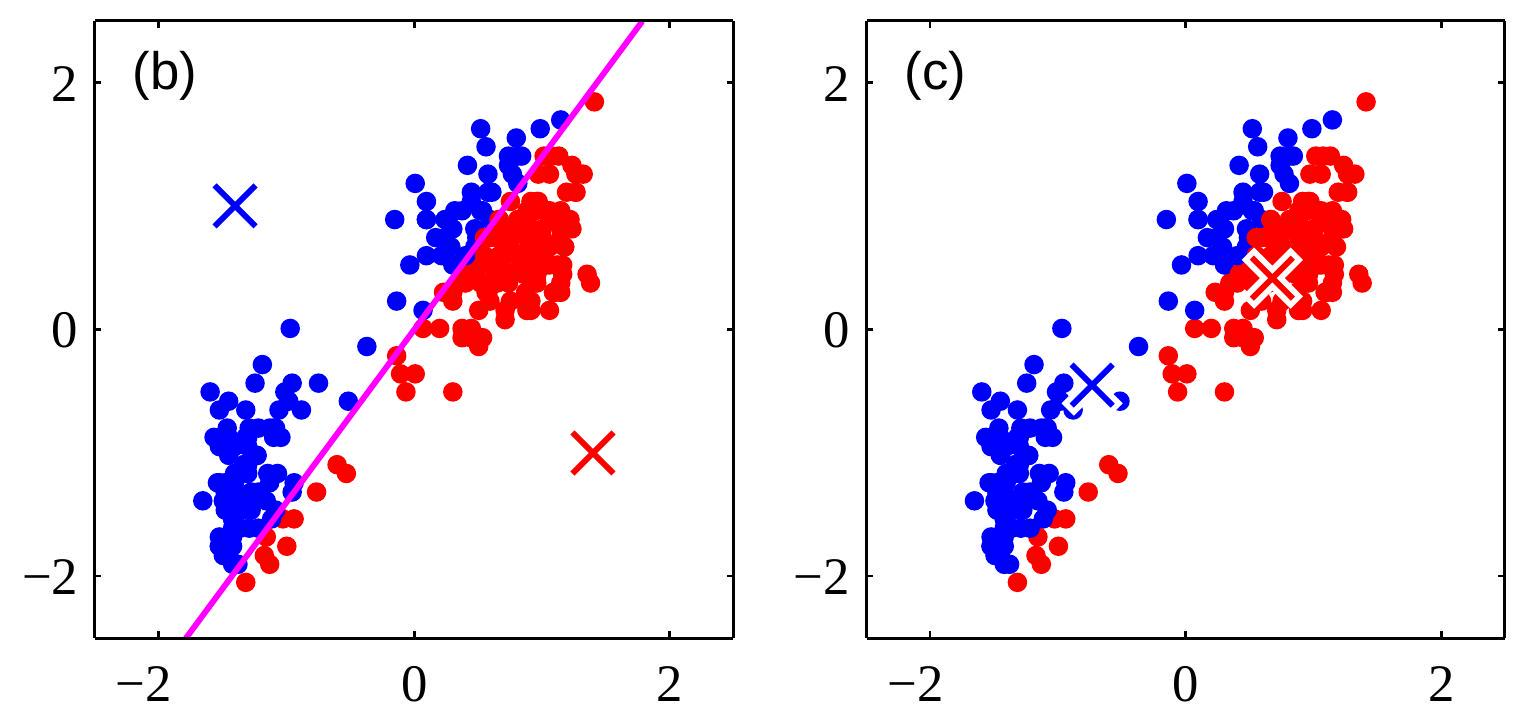
\includegraphics[max width=\textwidth, center]{2023_12_30_43b7e6c218cb987b5fcag-4}

\section*{Summary of K-means}
Initialize $\boldsymbol{\mu}_{k} \forall k$, then iterate:

\begin{enumerate}
  \item For all $n$, compute $\mathbf{z}_{n}$ given $\boldsymbol{\mu}$.
\end{enumerate}

$$
z_{n k}=\left\{\begin{array}{l}
1 \text { if } k=\arg \min _{j}\left\|\mathbf{x}_{n}-\boldsymbol{\mu}_{j}\right\|_{2}^{2} \\
0 \text { otherwise }
\end{array}\right.
$$

\begin{enumerate}
  \setcounter{enumi}{1}
  \item For all $k$, compute $\boldsymbol{\mu}_{k}$ given $\mathbf{z}$.
\end{enumerate}

$$
\boldsymbol{\mu}_{k}=\frac{\sum_{n=1}^{N} z_{n k} \mathbf{x}_{n}}{\sum_{n=1}^{N} z_{n k}}
$$

Convergence to a local optimum is assured since each step decreases the cost (see Bishop, Exercise 9.1).

\section*{Coordinate descent}
$\mathrm{K}$-means is a coordinate descent algorithm, where, to find $\min _{\boldsymbol{z}, \boldsymbol{\mu}} \mathcal{L}(\mathbf{z}, \boldsymbol{\mu})$, we start with some $\boldsymbol{\mu}^{(0)}$ and repeat the following:

$\mathbf{z}^{(t+1)}:=\arg \min _{\boldsymbol{z}} \mathcal{L}\left(\mathbf{z}, \boldsymbol{\mu}^{(t)}\right)$

$\boldsymbol{\mu}^{(t+1)}:=\arg \min _{\boldsymbol{\mu}} \mathcal{L}\left(\mathbf{z}^{(t+1)}, \boldsymbol{\mu}\right)$

\section*{Examples}
K-means for the "old-faithful" dataset (Bishop's Figure 9.1)

\begin{center}
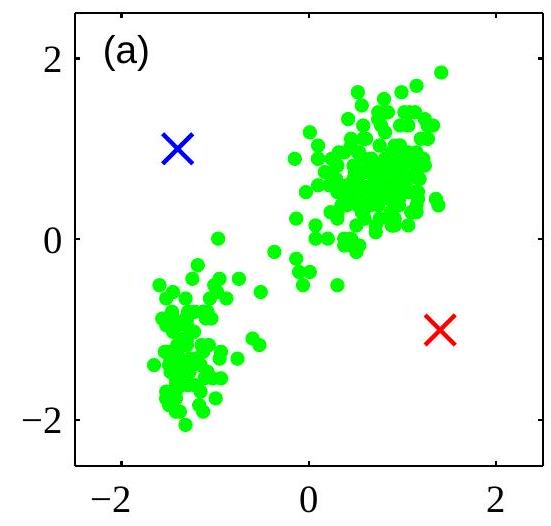
\includegraphics[max width=\textwidth]{2023_12_30_43b7e6c218cb987b5fcag-6(8)}
\end{center}

(e) Iteration 0

\begin{center}
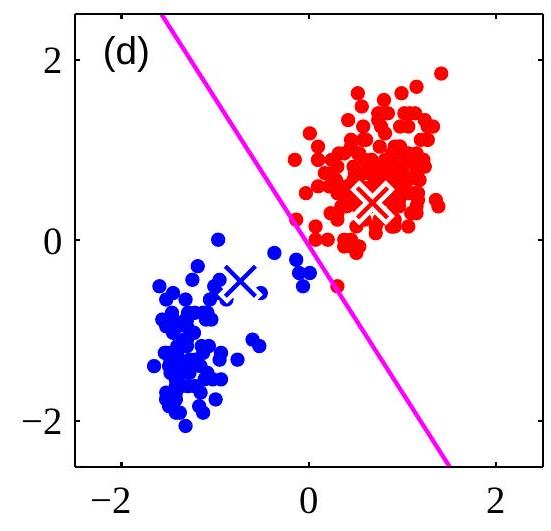
\includegraphics[max width=\textwidth]{2023_12_30_43b7e6c218cb987b5fcag-6(6)}
\end{center}

(h) Iteration 2

\begin{center}
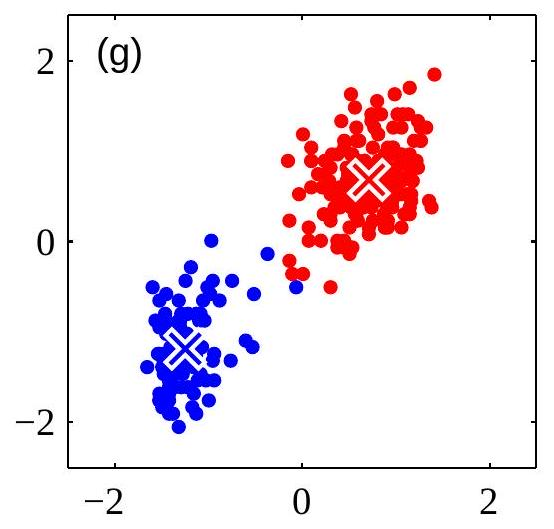
\includegraphics[max width=\textwidth]{2023_12_30_43b7e6c218cb987b5fcag-6(4)}
\end{center}

(k) Iteration 3

\begin{center}
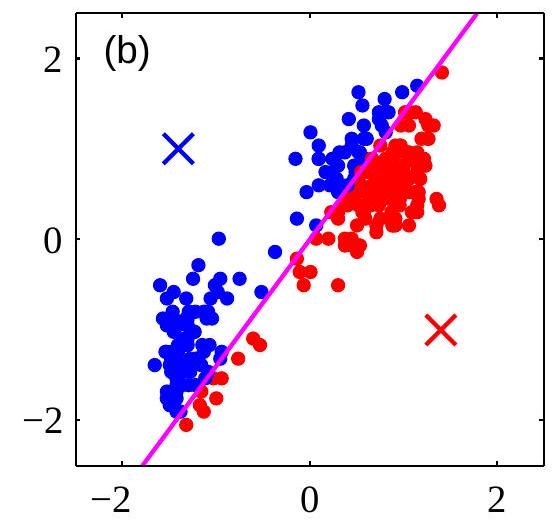
\includegraphics[max width=\textwidth]{2023_12_30_43b7e6c218cb987b5fcag-6(1)}
\end{center}

(f) Iteration 1

\begin{center}
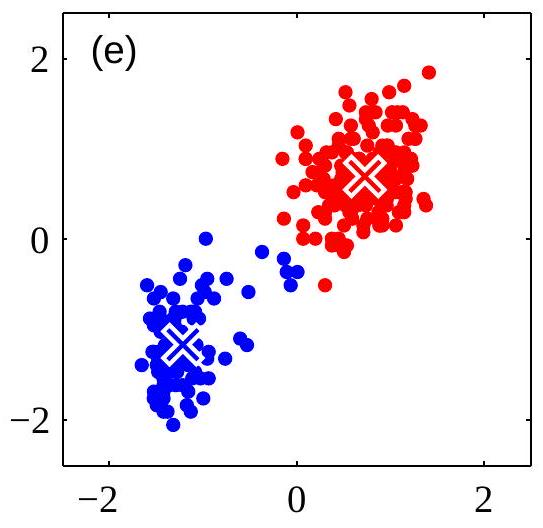
\includegraphics[max width=\textwidth]{2023_12_30_43b7e6c218cb987b5fcag-6}
\end{center}

(i) Iteration 2

\begin{center}
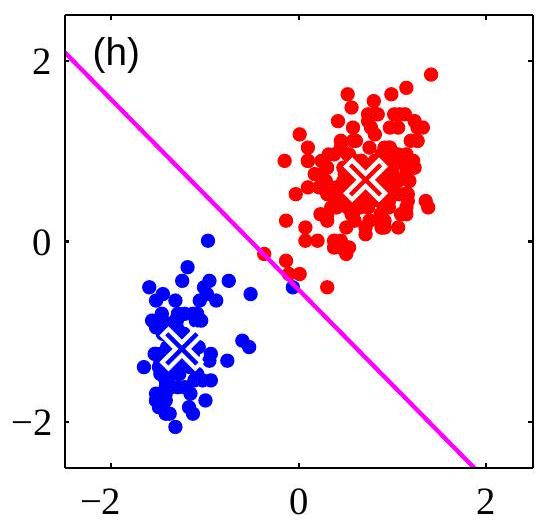
\includegraphics[max width=\textwidth]{2023_12_30_43b7e6c218cb987b5fcag-6(5)}
\end{center}

(l) Iteration 4

\begin{center}
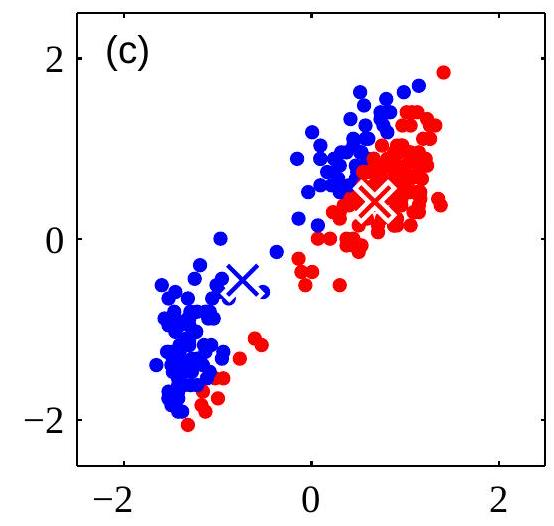
\includegraphics[max width=\textwidth]{2023_12_30_43b7e6c218cb987b5fcag-6(3)}
\end{center}

(g) Iteration 1

\begin{center}
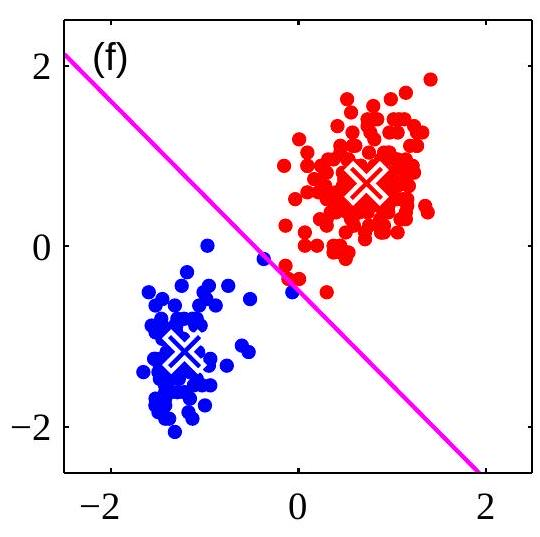
\includegraphics[max width=\textwidth]{2023_12_30_43b7e6c218cb987b5fcag-6(7)}
\end{center}

(j) Iteration 3

\begin{center}
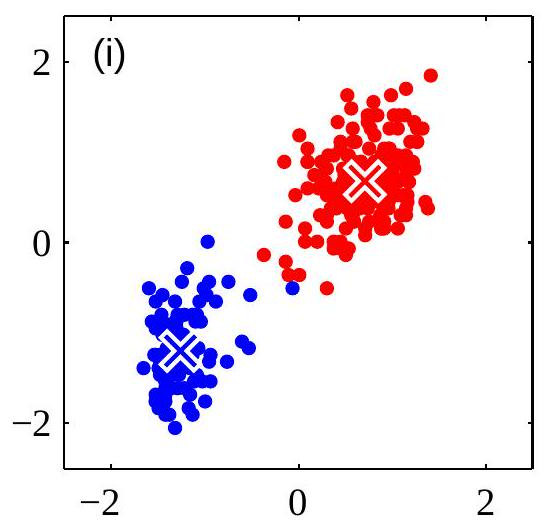
\includegraphics[max width=\textwidth]{2023_12_30_43b7e6c218cb987b5fcag-6(2)}
\end{center}

(m) Iteration 4

Data compression for images (this is also known as vector quantization).
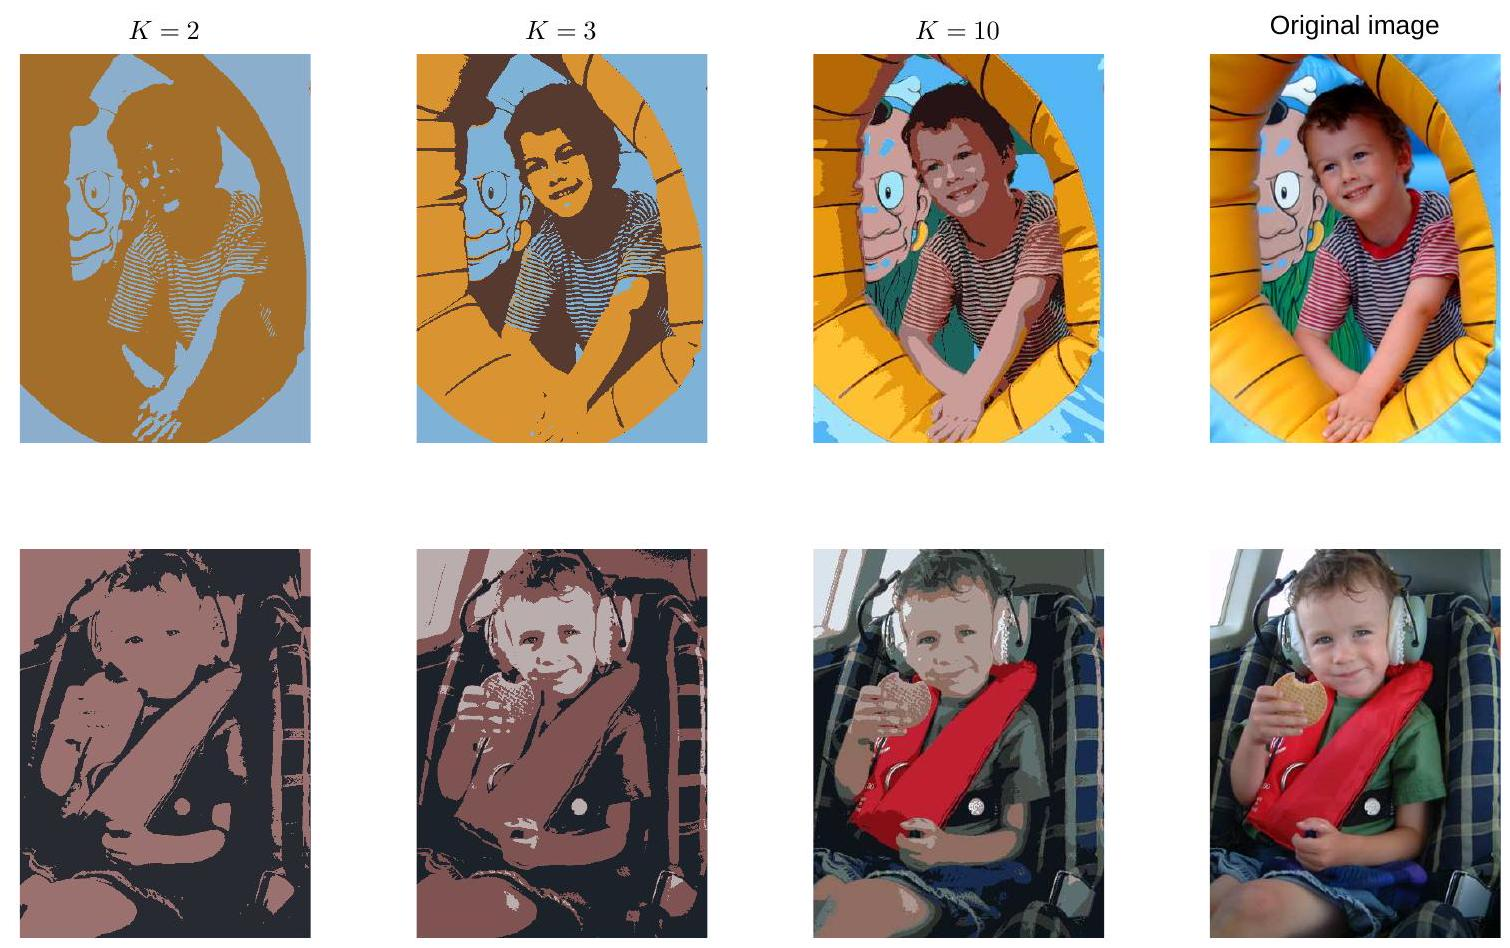
\includegraphics[max width=\textwidth, center]{2023_12_30_43b7e6c218cb987b5fcag-7}

\section*{Probabilistic model for K-means}
\section*{K-means as a Matrix Factorization}
Recall the objective

$\begin{aligned} \min _{\mathbf{z}, \boldsymbol{\mu}} \mathcal{L}(\mathbf{z}, \boldsymbol{\mu}) & =\sum_{n=1}^{N} \sum_{k=1}^{K} z_{n k}\left\|\mathbf{x}_{n}-\boldsymbol{\mu}_{k}\right\|_{2}^{2} \\ & =\left\|\mathbf{X}^{\top}-\mathbf{M} \mathbf{Z}^{\top}\right\|_{\text {Frob }}^{2}\end{aligned}$

s.t. $\boldsymbol{\mu}_{k} \in \mathbb{R}^{D}$,

$$
z_{n k} \in\{0,1\}, \sum_{k=1}^{K} z_{n k}=1
$$

\section*{Issues with K-means}
\begin{enumerate}
  \item Computation can be heavy for large $N, D$ and $K$.

  \item Clusters are forced to be spherical (e.g. cannot be elliptical).

  \item Each example can belong to only one cluster ("hard" cluster assignments).

\end{enumerate}

\end{document}